
\chapter{Implementation}\label{section:implementation}

\section{Overview of Important Class Diagrams}

As stated in section~\ref{section:aims}, this project extends from SICSA project which uses only publications as expertise evidence.
The aim of this project is to integrate funded projects with publications to improve the performance of the retrieval system.
Figure~\ref{fig:classDiagram1} shows the relationship between Candidate (Expert), Project, Publication and University classes. Each component in the figure
shows only important attributes and methods. The Candidate class represents an expert who lectures at a university and has a set of publications and projects.
\begin{figure}
\centering
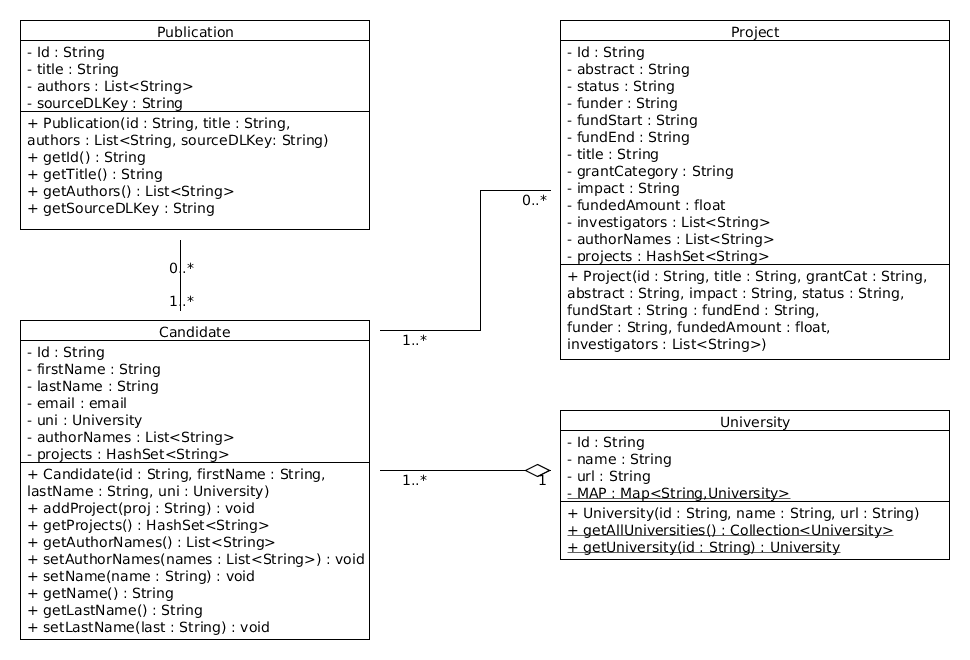
\includegraphics[scale=0.4]{./figures/classDiagram1.png}
\caption{Class Diagram} \label{fig:classDiagram1} 
\end{figure}

\begin{figure}
\centering
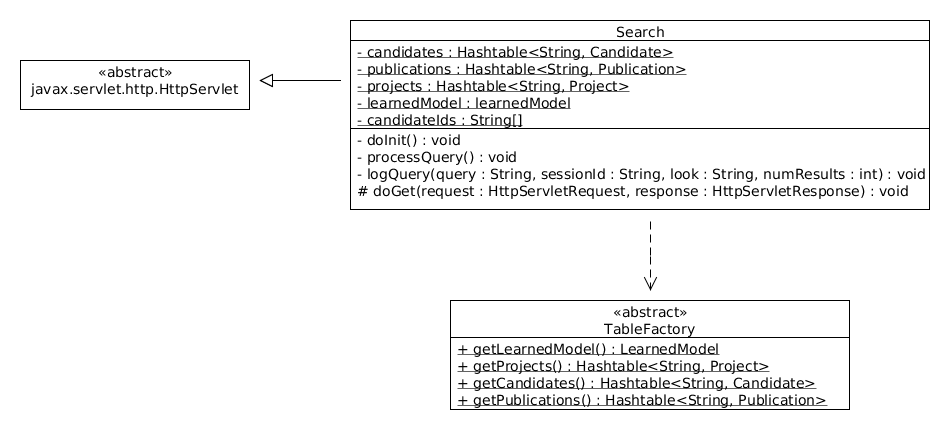
\includegraphics[scale=0.4]{./figures/tablefactory.png}
\caption{TableFactory Class Diagram} \label{fig:tableFactory} 
\end{figure}

Figure~\ref{fig:tableFactory} shows class diagrams of \textit{TableFactory}, and \textit{Search}. These two components can also be viewed as the core
part of the system. The responsibility of each class is given below:
\begin{itemize}
 \item \textit{Search} extends Java Servlet which handles search request submitted by a user.
 \item \textit{TableFactory} loads Experts, Publications, and Projects stored in a file and send them to Search Servlet.
\end{itemize}

\textit{Search} contains 4 important methods as follows: 
\begin{itemize}
 \item \textit{doInit()} loads AcademTechQuerying component for querying.
 \item \textit{processQuery()} processes a query obtained by a user. More details are given in section~\ref{section:applyinglearnedmodel}.
 \item \textit{logQuery()} saves a query to a log file.
 \item \textit{doGet()} handles a GET request when user submits a query. It also generates HTML page of the query results.
\end{itemize}

As stated in section ~\ref{section:goodexpert}, the features extracted from funded projects and publications of each expert will be used in Learning to Rank
to improve the retrieval performance of the system. But before we get to Learning to Rank, first of all, we need to understand
AcademTechQuerying Class and RetrievedResults Class which are components used in retrieving results with respect to a query. 
\begin{figure}
\centering
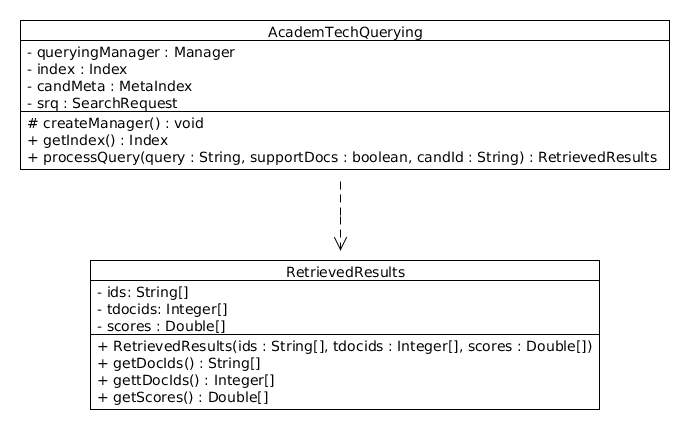
\includegraphics[scale=0.3]{./figures/AcademTechQuerying.png}
\caption{AcademTechQuerying Class and RetrievedResults Class} \label{fig:AcademTechQuerying} 
\end{figure}



Figure~\ref{fig:AcademTechQuerying} shows class diagrams of AcademTechQuerying and RetrievedResults. As stated in section~\ref{section:terrier},
the search engine platform used in this project is Terrier. It handles indexing and retrieval processes discussed in section~\ref{section:IRarchitecture}.
The AcademTechQuerying Class makes use of 2 Terrier components as follows:  
\begin{itemize}
 \item \textit{queryingManager} of type Manager, responsible for handling/co-ordinating the main high-level operations of a query.
 \item \textit{srq} of type SearchRequest, responsible for retrieving search result from Manager.
\end{itemize}
The most important method of AcademTechQuerying is processQuery(). It returns RetrievedResults component. This method takes a query string, supportDocs and candId as arguments. The first argument tells
the system that a query is used to retrieve the result, the second and third arguments are used in case the system wants documents associated to a candidate 
with respect to a query.

The RetrievedResults Class has 3 attributes as follows:
\begin{itemize}
 \item \textit{ids}, an array of String, which is the ids of the documents(in this case, ids of experts) retrieved by the system.
 \item \textit{tdocids}, an array of Integer, which is the ids used by Terrier
 \item \textit{scores}, an array of Double, which is the scores of each document retrieved by the system.
\end{itemize}

\section{Data Extraction}\label{sec:dataextraction}
\begin{figure}
\centering
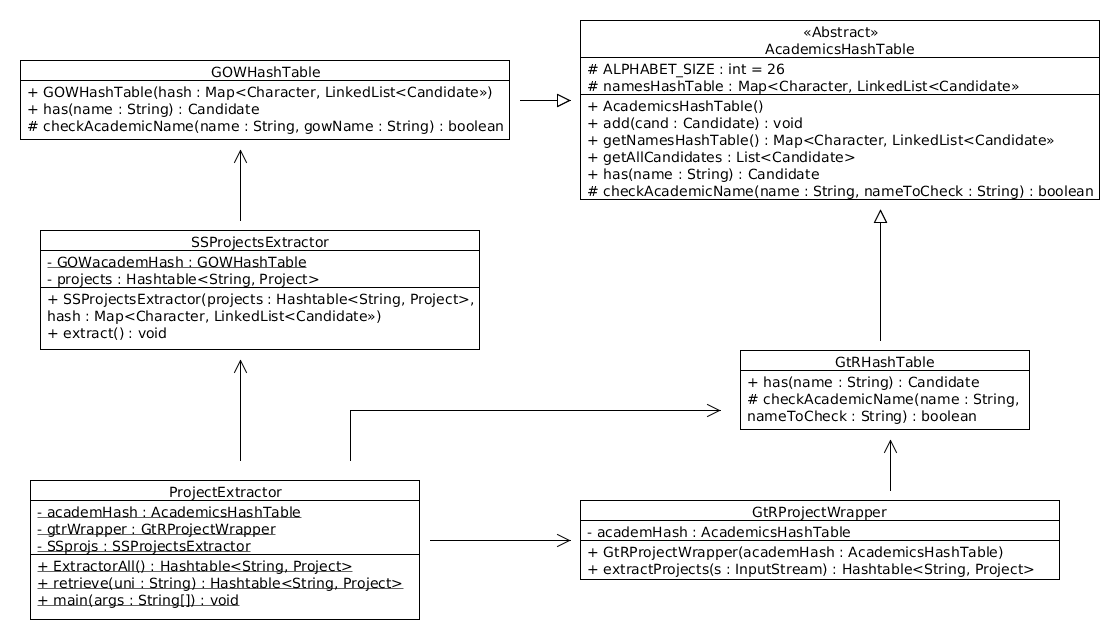
\includegraphics[scale=0.35]{./figures/projectsExtraction.png}
\caption{Projects Extraction Class Diagrams} \label{fig:projectsExtraction} 
\end{figure}
In section~\ref{section:aims}, it was stated that funded projects are obtained from Grant on the Web~\cite{gow} and Research Councils UK~\cite{gtr}.
This section shows classes used to extract funded projects from each source and gives statistics regarding the number of funded projects from each source.
Figure~\ref{fig:projectsExtraction} shows class diagram related to projects extraction task.

\begin{itemize}
 \item \textbf{AcademicsHashTable} is an abstract class which makes use of HashMap data structure, \\ 
 $Map<Character, LinkedList<Candidate>>$, for efficient look up when matching candidate to our
known candidates. It is keyed by the first character of candidate's name. There are 2 abstract methods in this class: has() and checkAcademicName() methods.
Both of them are used together to check if the candidate is matched to our known candidates.
\item \textbf{GtRHashTable} extends from the abstract class AcademicsHashTable. The purpose of this class is the same as AcademicsHashTable Class but
implements has() and checkAcademicName() methods which are applicable in Research Councils UK~\cite{gtr} data source.
\item \textbf{GOWHashTable} extends from the abstract class AcademicsHashTable. Its purpose is similar to AcademicsHashTable Class but
has different implementations of has() and checkAcademicName() methods to GOWHashTable's which are applicable in Grant on the Web~\cite{gow} spreadsheet data source.
\item \textbf{SSProjectsExtractor} is a class that makes use of GOWHashTable Class to extract funded projects from Grant on the Web~\cite{gow} spreadsheet.
\item \textbf{GtRProjectWrapper} is a class used GOWHashTable Class to extract funded projects from Research Councils UK~\cite{gtr}.
\item \textbf{ProjectExtractor} is a class that makes use of SSProjectsExtractor and GtRProjectWrapper Classes to extract funded projects from both sources.
\end{itemize}

Since each source records expert's name in different formats. For example, Prof. Joemon Jose may be recorded Jose JM in one source and Jose J in another,
Polymorphism~\cite{polymorphism} (in this case, different implementations of has() and checkAcademicName() methods between GtRHashTable and GOWHashTable) is required.
However, pattern matching between
expert's names in Grant on the Web~\cite{gow} spreadsheet is still impossible as this source records in the following format: 
[lastname], [role] [the first and/or second letter of name] such as Rogers, Dr. Simon. The problem occurs with experts, Dr. Craig Macdonald lecturing at
University of Glasgow and Prof. Catriona Macdonald lecturing at Glasgow Caledonian University
as the source records Macdonald, Dr C for the former and Macdonald, Professor C for the latter. Although, role might be used to distinguish between them but
for some experts the role is not known and there might be the situation that the role is also the same. 
Therefore, university is used as part of the matching as well.

\begin{table}
\centering
\scalebox{0.5}{\begin{tabular}{|c|c|}
\hline \textbf{Source} & \textbf{Number of Funded Projects} \\
\hline Grant on the Web & 32 \\
\hline Research Councils UK & 337 \\
\hline   & 369 total \\ 
\hline
\end{tabular}
}
\caption{The number of funded projects extracted from each source} \label{table:stats}
\end{table}
Figure ~\ref{table:stats} shows the number of funded projects extracted from each source. There are 1569 known candidates in the system.

\section{Indexing}

Before indexing process begins, the system has to generate data in TREC format and an association file between TREC files. \textbf{FileGenerator} class
handles this. It includes only 1 method main(). The list below is files generated by the class:
\begin{itemize}
 \item ContactsList.trec.gz
 \item Homepages.trec.gz
 \item Projects.trec.gz
 \item Publications.trec.gz
 \item association.txt
\end{itemize}

\paragraph{ContactsList.trec.gz} \hspace{0pt} \\
This file compressed in gz format stores a list of experts in TREC format. Each expert's data is recorded in the following format:
\begin{verbatim}
<DOC>
	<DOCNO>expert's id</DOCNO>
	<name>expert's name</name>
	<snippets>description of expert</snippets>
	<keyTerms></keyTerms>
	<uni>expert's university</uni>
	<uniId>university's id</uniId>
	<location>location of the university</location>
	<role>role of the expert</role>
	<pubGroup>group of publication</pubGroup>
	<conference>conference's name involved</conference>
	<journal>type of journal</journal>
	<coauthorGroup>group of coauthor</coauthorGroup>
</DOC>
\end{verbatim}

\paragraph{Homepages.trec.gz} \hspace{0pt} \\
This file compressed in gz format stores a list of home pages in TREC format. Each home page associated to one expert is recorded in the following format:
\begin{verbatim}
 <DOC>
        <DOCNO>homepage's id</DOCNO>
        <candidate>expert's id</candidate>
        <content>content of the home page</content>
</DOC>
\end{verbatim}


\paragraph{Projects.trec.gz} \hspace{0pt} \\
This file compressed in gz format stores a list of funded projects in TREC format. Each funded project is recorded in the following format:
\begin{verbatim}
<DOC>
	<DOCNO>funded project's id</DOCNO>
	<type>type of evidence</type>
	<title>title of the project</title>
	<grantCategory>type of grant</grantCategory>
	<start>start date</start>
	<end>end date</end>
	<abstract>abstract of the project</abstract>
	<impact>impact of the project</impact>
	<people>
		<person>expert's name</person>
	</people>
</DOC>

\end{verbatim}
where \textit{$<$type$>$} tag's value is always \textit{proj} which tells Terrier that this document is of type \textit{proj}. This tag is very useful when 
the system transforms the query to retrieve documents using only funded projects as expertise evidence (see section~\ref{section:union}).

\paragraph{Publications.trec.gz} \hspace{0pt} \\
This file compressed in gz format stores a list of publications in TREC format. Each publication is recorded in the following format:
\begin{verbatim}
 <DOC>
        <DOCNO>publication's id</DOCNO>
        <TYPE>type of evidence</TYPE>
        <type>inproceedings</type>
        <pubtitle>title</pubtitle>
        <author>author's name 1</author>
        <author>author's name 2</author>
        <conference>conference's name involved</conference>
        <year>year</year>
        <snippets>description of the publication</snippets>
        <keyTerms></keyTerms>
        <citationContexts></citationContexts>
        <uni>university's name</uni>
        <uniId>university's id</uniId>
        <location>location of the university</location>
        <role>role of the project</role>
        <pubGroup>group of the publication</pubGroup>
        <journal>type of journal</journal>
        <coauthorGroup>group of coauthor</coauthorGroup>
</DOC>
\end{verbatim}
There are 2 \textit{$<$type$>$} tags whose values are always set to \textit{pub} and \textit{inproceedings}. The idea is similar one's in 
funded project which is for filter modes in Terrier.

\paragraph{association.txt} \hspace{0pt} \\
This file tells Terrier about the associations between experts, publications, and funded projects. It is stored in the following format:
\begin{verbatim}
 expert_id expert_homepage pub_id1 pub_id2 ... pub_idn proj_id1 
 proj_id2 ... proj_idn expert_homepage_id
\end{verbatim}
where one line in the file corresponds to only one expert.

Once all the files have been generated, Terrier indexes those files. Table~\ref{table:newtstats} shows statistics of new system after indexing.

\begin{table}
\centering
\scalebox{0.5}{\begin{tabular}{|c|c|}
\hline Number of experts & 1569 \\
\hline Number of all documents   & 25311 \\ 
\hline Number of tokens (terms) & 6976895 \\
\hline
\end{tabular}
}
\caption{Statistics of New System After Indexing Process} \label{table:newtstats}
\end{table}



\section{Producing a Learned Model}\label{section:producelearnedmodel}
Section ~\ref{sec:learnedmodel} described general steps in producing a learned model. This section aims to discuss classes involved in producing a learned model.
As section~\ref{sec:learnedmodel} suggested, the first step in producing a learned model is to generate a set of training queries. 
Then all features described in Section~\ref{section:goodexpert} for each document (expert) with respect to each training query are extracted and saved
in a file. This file in learning to rank is called LETOR file (see section~\ref{sec:letorFile}).
Figure~\ref{fig:sampleletorfile} is a LETOR file. There are 7 features as described section~\ref{section:goodexpert}.

\begin{figure}
\centering
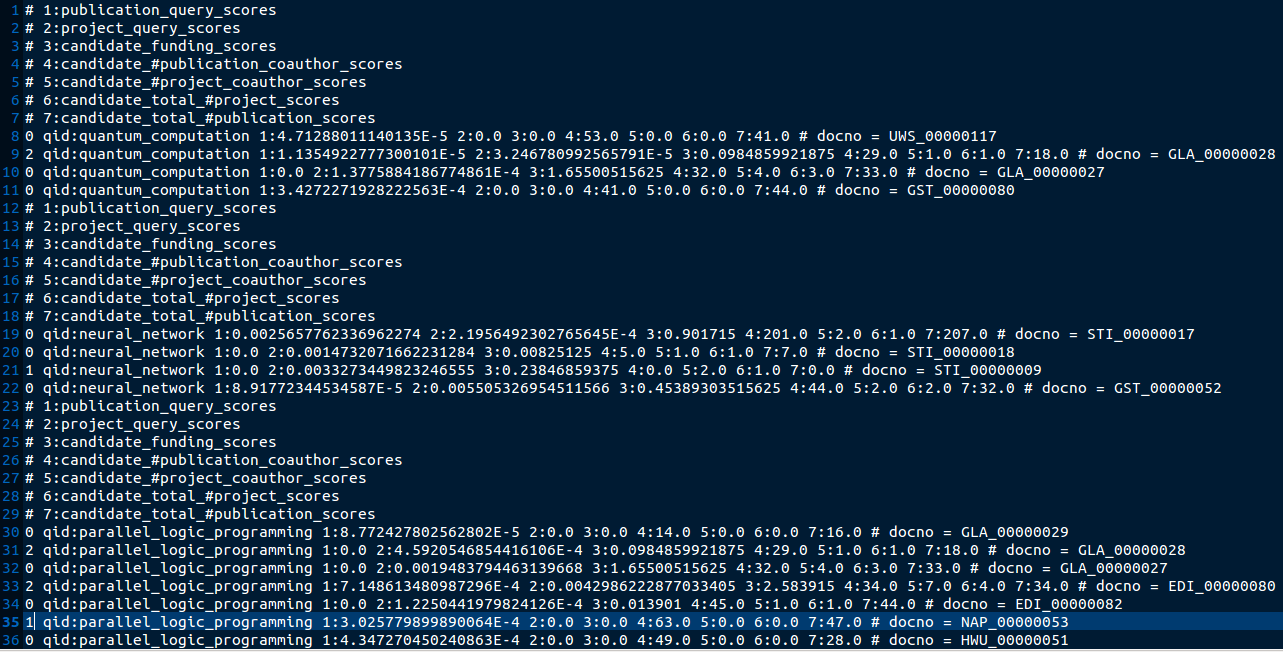
\includegraphics[scale=0.3]{./figures/sampleletorfile.png}
\caption{LETOR file of Training Queries} \label{fig:sampleletorfile} 
\end{figure}

\begin{figure}
\centering
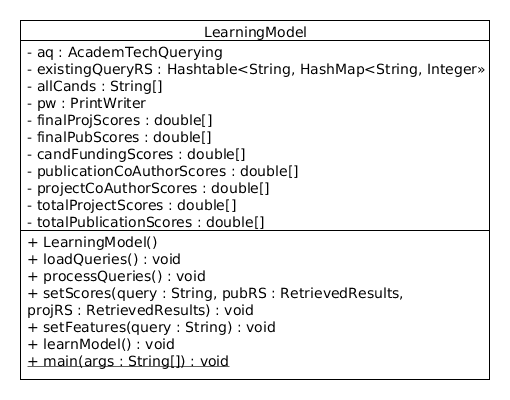
\includegraphics[scale=0.7]{./figures/learningModel.png}
\caption{Class Diagram of LearningModel} \label{fig:learningmodel} 
\end{figure}

Figure ~\ref{fig:learningmodel} shows a class diagram that is used to produce a learned model. There are 5 important methods as follows
\begin{itemize}
 \item \textit{loadQueries()} is a method that loads all training queries from a file.
 \item \textit{processQuery()} is a method that retrieve documents (experts) with respect to publication query and project query.
 \item \textit{setScores()} is a method that performs a union between results with respect to publication query and project query as discussed in Section ~\ref{section:union}
 \item \textit{setFeatures()} is a method that extracts features for each document (expert) and write into a LETOR file.
 \item \textit{learnModel()} is a method that produces a learned model using RankLib.
\end{itemize}

As stated in Section~\ref{section:rankLib}, learning to rank algorithms used in this project are AdaRank and Coordinate Ascent. The performance of each
of them will be discussed in Evaluation Section. Figures~\ref{fig:samplemodel} and~\ref{fig:adarankModel} show learned models 
using \textit{Coordinate Ascent} and \textit{AdaRank} Algorithms.
Section~\ref{section:applyinglearnedmodel} will explain a component used to apply a learned model.

\begin{figure}
\centering
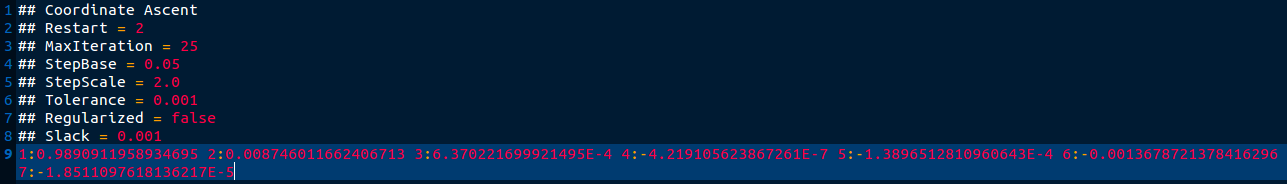
\includegraphics[scale=0.3]{./figures/samplemodel.png}
\caption{Learned Model Using Coordinate Ascent Algorithm} \label{fig:samplemodel} 
\end{figure}

\begin{figure}
\centering
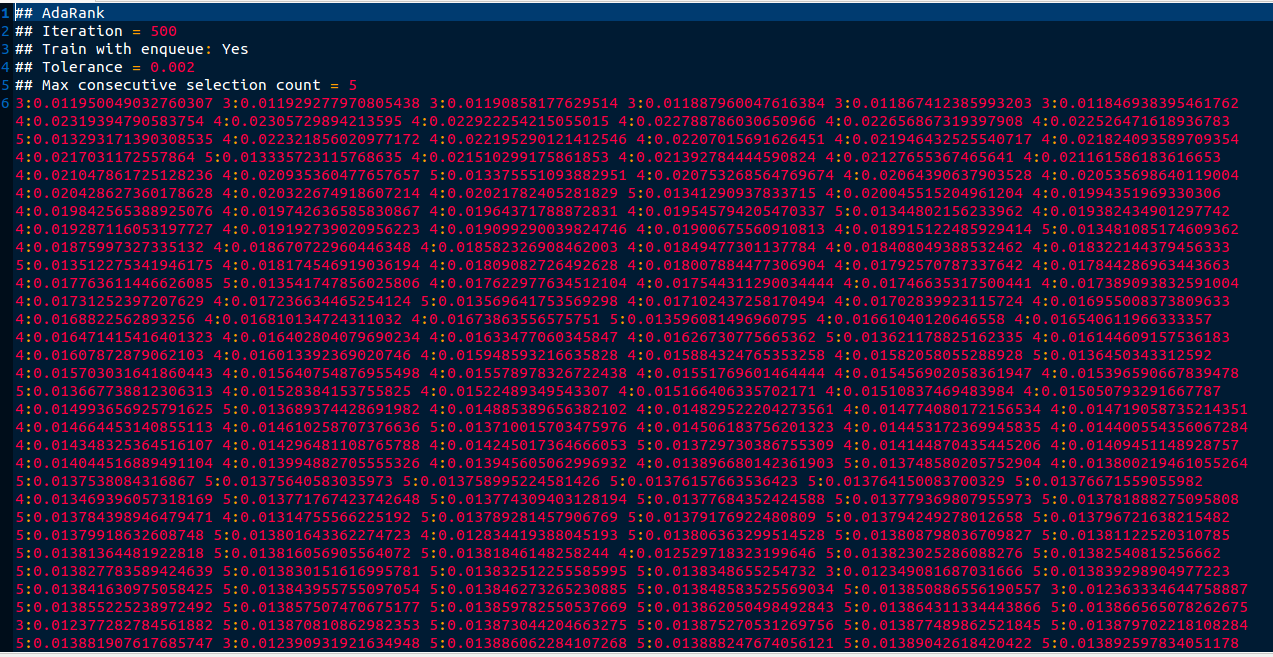
\includegraphics[scale=0.3]{./figures/adarankModel.png}
\caption{Learned Model Using AdaRank Algorithm} \label{fig:adarankModel} 
\end{figure}

\section{Applying a Learned Model}\label{section:applyinglearnedmodel}
In section~\ref{sec:background_applyLearnedModel}, we explained the process of applying a learned model. This section aims to describe components
that handle this task. The class \textit{CandidateScores} has a method called, getTotalScore() taking a learnedModel component as a parameter. 
This method applies a learned model as described in section~\ref{sec:background_applyLearnedModel} and returns a score associated with an expert.
Figure~\ref{fig:scoreandsorting} shows class diagrams of \textit{Candidatescores} and \textit{LearnedModel}.

\begin{figure}
\centering
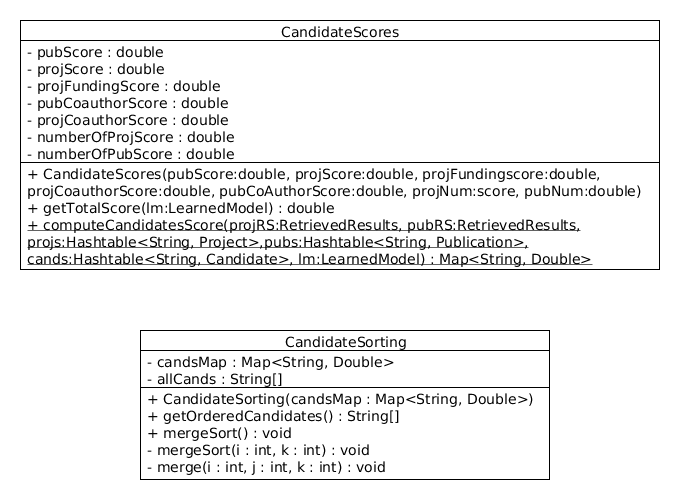
\includegraphics[scale=0.3]{./figures/score&sorting.png}
\caption{Class Diagrams of CandidateScores and CandidateSorting} \label{fig:scoreandsorting} 
\end{figure}

\begin{figure}
\centering
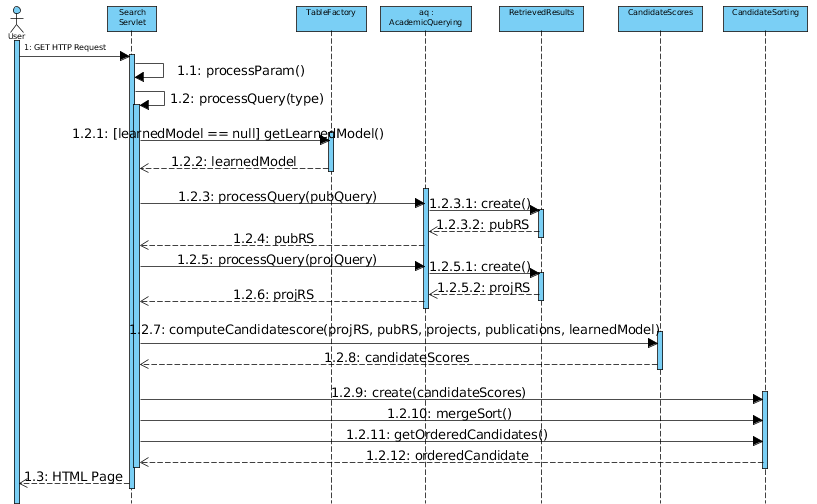
\includegraphics[scale=0.4]{./figures/searchsequence.png}
\caption{Sequence Diagram of Querying} \label{fig:searchsequence} 
\end{figure}

Figure~\ref{fig:searchsequence} illustrates a sequence diagram of querying. This sequence diagram only shows important processes to retrieve
relevant results. Given a query submitted by a user, Search servlet processes parameters sent via GET request by calling processParam() method. This is
followed by invoking processQuery() method which takes one parameter, ``type''. This parameter is used for filter mode. The method processQuery() 
performs tasks discussed in section~\ref{section:union}.
The \textit{CandidateScores} is used for computing scores of candidates based on a learned model. The \textit{CandidateSorting}
sorts scores of candidates obtained after applying a learned model in descending score as discussed in section~\ref{sec:learnedmodel}.
The sorting algorithm applied in this class is \textbf{merge sort}~\cite{mergesort}, giving time complexity of $O(n\cdot log\, n)$ where $n$ is the 
number of documents (experts) to be sorted.
Figure~\ref{fig:scoreandsorting} shows class diagrams of \textit{CandidateScores}, \textit{LearnedModel} and \textit{CandidateSorting}.
Important attributes and methods are only shown.


\section{User Interface of New System}

\begin{figure}
 \centering
 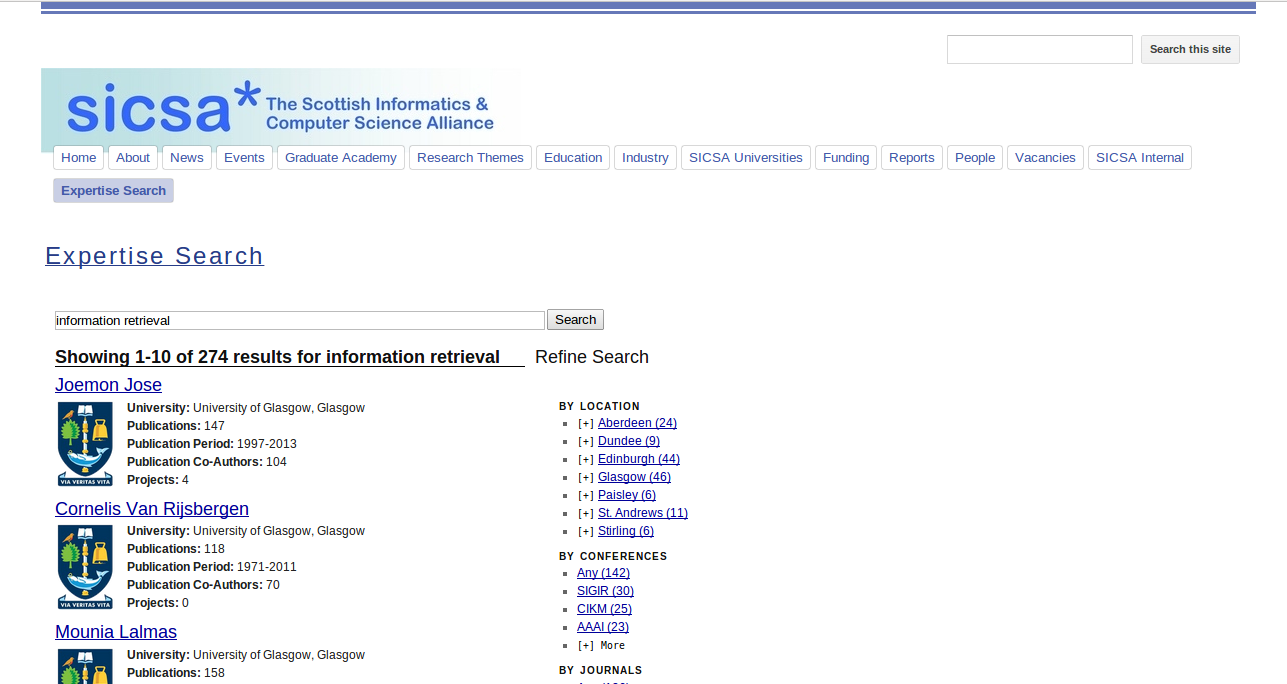
\includegraphics[width=13cm,height=15cm,keepaspectratio]{./figures/newsearch.png}
 \caption{New Facets : Experts In Response to ``information retrieval'' Query} \label{fig:newsearch} 
 \end{figure}
 Figure~\ref{fig:newsearch} shows a new search facet in response to a query ``information retrieval''. The number of 
projects experts have been involved in is displayed. In addition to the current system filter modes, filter options by using projects, publications and both
expertise evidence, and by projects' total funding are added on the right panel of the page.

 \begin{figure}
 \centering
 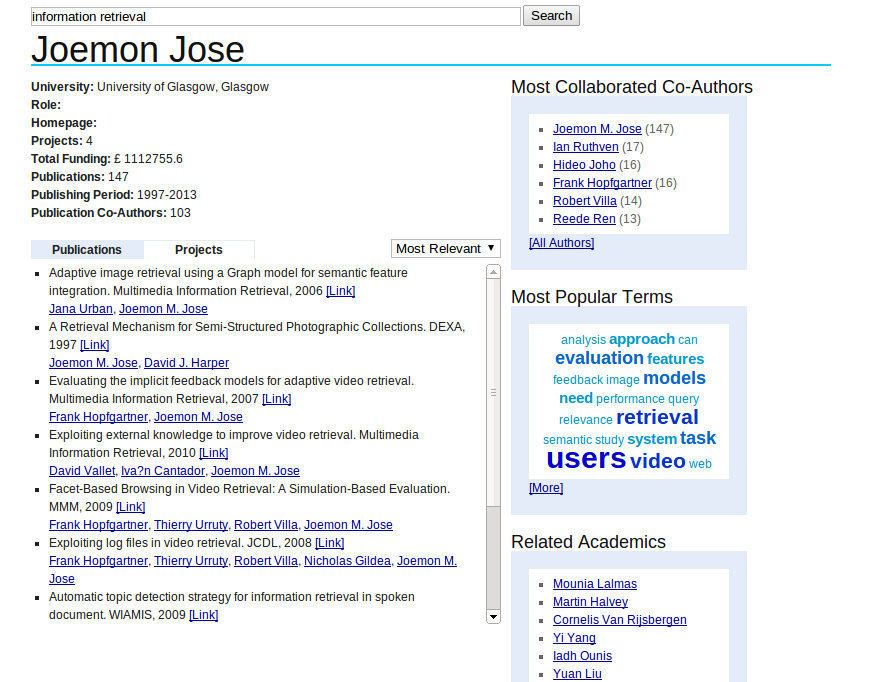
\includegraphics[width=13cm,height=15cm,keepaspectratio]{./figures/newProfilePagePublication.png}
 \caption{New Expert's Profile Facet} \label{fig:newProfilePage} 
 \end{figure}
 Figure~\ref{fig:newProfilePage} shows a new facet of profile page. There are 2 tabs for publications and funded projects and a drop down box for selecting
 result filter modes. The number of projects, project collaborators, project period and total funding are shown.
 
 \begin{figure}
 \centering
 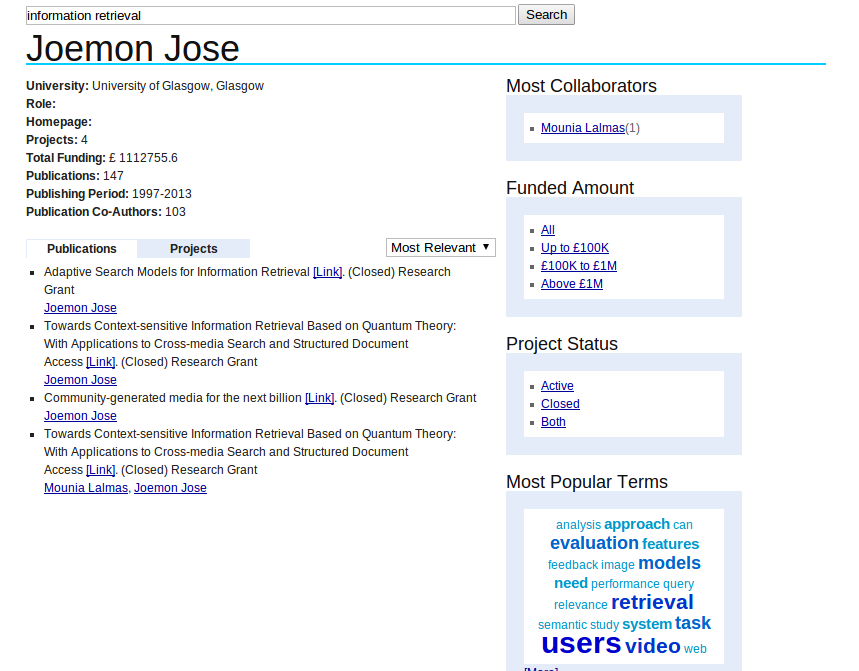
\includegraphics[width=13cm,height=15cm,keepaspectratio]{./figures/newPofilePageProject.png}
 \caption{Project Tab} \label{fig:newPofilePageProject} 
 \end{figure}
 Figure~\ref{fig:newPofilePageProject} shows a facet when a project tab is selected. The right hand side of the page shows the most project collaborators
 and other filter modes: filter projects by amount of funding and by the status of projects.
 
 \begin{figure}
 \centering
 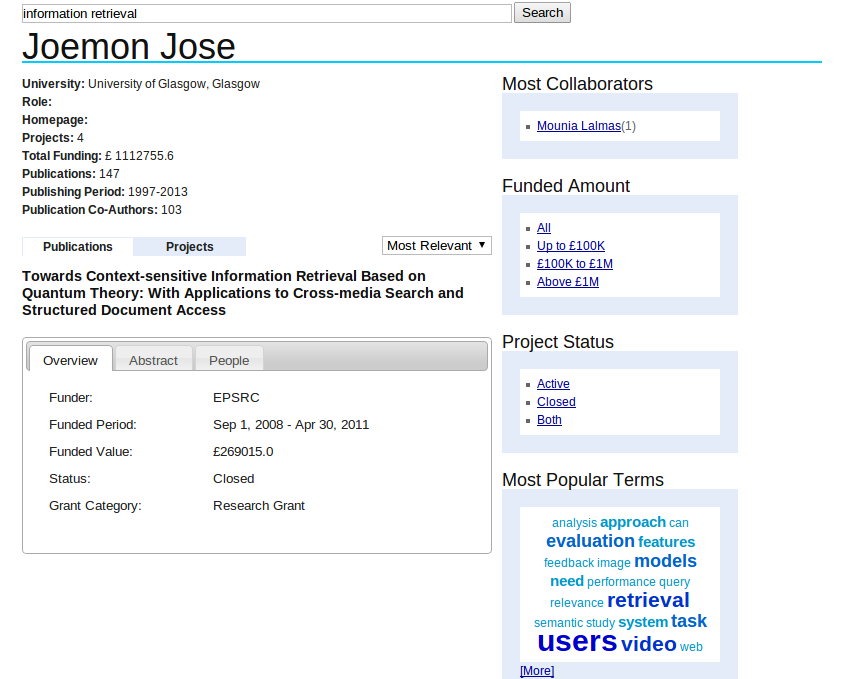
\includegraphics[width=13cm,height=15cm,keepaspectratio]{./figures/newProfileSelectedProject.png}
 \caption{Project Page} \label{fig:newProfileSelectedProject} 
 \end{figure}
 
 Figure~\ref{fig:newProfileSelectedProject} shows a facet when user selects a project link. This shows descriptions of a selected project.
 The descriptions include:
 \begin{itemize}
  \item Funder
  \item Title
  \item Funded Value
  \item Funded Period
  \item Status
  \item Grant Category
  \item People involved in the project
  \item Abstract
  \item Impact
 \end{itemize}
 Some projects descriptions are not shown if they are missing.




